\documentclass[11pt]{article}

\usepackage[utf8]{inputenc}
\usepackage[margin=1in]{geometry}  % Adjust page margins
\usepackage{graphicx}              % For including images (PDF, PNG, JPG)
\usepackage[inkscapelatex=false]{svg}
\usepackage{listings}              % For including code
\usepackage{xcolor}                % For custom colors
\usepackage{hyperref}              % For hyperlinks in the PDF
\usepackage{amsmath, amssymb, amsthm} % For math symbols and environments
\usepackage{mathrsfs}
\usepackage{enumitem}
\geometry{a4paper, margin=1in} % Set margin to 1 inch
\usepackage{fancyhdr} % For header and footer
\usepackage{hyperref} % For clickable links in the PDF
\usepackage{array} % For table column formatting
\usepackage{times} % Uses Times font for the text
\usepackage{float}

\title{CMOR 421/521 Assignment 2: OpenMP}
\author{Yuhao Liu}
\date{\today}

% --------------------------------------------------------------------------------
% Customize the appearance of code listings (for C++ syntax).
% --------------------------------------------------------------------------------
\lstdefinestyle{C++Style}{
    language=C++,
    basicstyle=\small\ttfamily,
    keywordstyle=\color{blue}\bfseries,
    commentstyle=\color{gray},
    stringstyle=\color{magenta},
    numbers=left,
    numberstyle=\tiny,
    stepnumber=1,
    breaklines=true,
    tabsize=4,
    showstringspaces=false
}

% If you store SVG images in a subfolder, specify the path here. 
% e.g.: \svgpath{{../images/}}
\svgpath{{./}}

\begin{document}

\maketitle

\tableofcontents
\bigskip

\newpage

\section{Directory Structure}
Below is my file organization for this assignment. 
My final zip file follows this structure (driver files in the top-level directory, 
\texttt{docs/} for LaTeX, \texttt{src/} for source files, and \texttt{include/} for header files):

\begin{figure}[H]
    \centering
    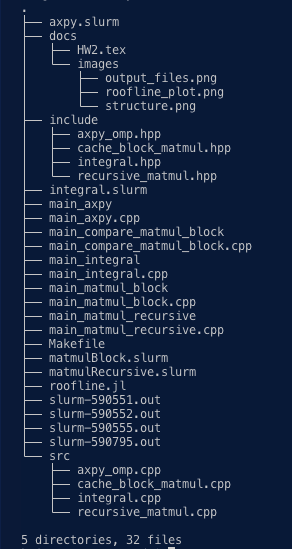
\includegraphics[width=0.3\linewidth]{Assignments/HW1/docs/images/structure.png}
    \caption{structure}
    \label{fig:structure}
\end{figure}

\begin{itemize}
    \item The \verb|main_mutiplication.cpp| and \verb|main_transpose.cpp| are include \verb|main| function for matrix transpose and matrix multiplication in naive method, cache-block method, and recursive method. 
    \item The \verb|main_mutiplication_col.cpp| is used to test when $A^T$ is stored in column major format, the performance for different methods.
    \item The \verb|visualize_mutiplixation.jl| and \verb|visualize_transpose.jl| are Julia code for plot the figures.
    \item The folder \verb|Env_HW1| are the Julia project local environment. You need to use the following command in terminal for execute these files. First,
    \begin{verbatim}
        cd ./HW1
    \end{verbatim}
    and using \verb|]| to enter the environment space, and then using command \verb|activate Env_HW1| to load the local environment. You can also use \verb|st| to check what library I used.
    \item The folder \texttt{docs/} is to store the Latex file and images.
    \item The folder \texttt{include/} is the place for \verb|.hpp| files. The \verb|matrix_transpose.hpp| and \verb|matrix_multiplication.hpp| are in there.
    \item The folder \texttt{src/} is the place for \verb|matrix_transpose.cpp| and \verb|matrix_multiplication.cpp| which are used to implemented all different methods for matrix transpose, matrix multiplication, and the timing analysis functions.

\end{itemize}

\newpage

\section{How to Build and Run the Code}
\label{sec:build_run}
\begin{itemize}
    \item \textbf{Build Instructions:} 
        \begin{itemize}
            \item For matrix transpose, you can use
            \begin{verbatim}
                make matrix_transpose_02
            \end{verbatim}
            and
            \begin{verbatim}
                make matrix_transpose_03
            \end{verbatim}
            to compile the program with \verb|-O2| or \verb|-O3| optimization flags.
            \item For matrix multiplication, you can use
            \begin{verbatim}
                make matrix_multiplication_02
            \end{verbatim}
            and
            \begin{verbatim}
                make matrix_multiplication_03
            \end{verbatim}
            to compile the program with \verb|-O2| or \verb|-O3| optimization flags.
            \item For the matrix transpose test when $A^T$ is stored column major, you can use
            \begin{verbatim}
                g++ -std=c++17 -O3 main_transpose_col.cpp -o main_transpose_col
            \end{verbatim}
            to compile.
        \end{itemize}
    \item \textbf{Running Instructions:} 
    
        Once you build the execution file, it will appear as driver files. You can use the following command to run the code:
        \begin{verbatim}
            ./matrix_transpose_02
            ./matrix_transpose_03
            ./matrix_multiplication_02
            ./matrix_multiplication_03
            ./main_transpose_col
        \end{verbatim}
    \item  \textbf{Execution: }
        When you execute the program, in the terminal you can see the output like the following figure:
        \begin{figure}[H]
            \centering
            \includegraphics[width=0.5\linewidth]{Assignments//HW1//docs//images/method_accuracy.png}
            \caption{Method accuracy}
            \label{fig:Method accuracy}
        \end{figure}
        This will check that the relative error for each matrix transpose implementation is zero up to machine precision.

        After you run one of above command, you will see there are two new folders \texttt{obj/} and \texttt{result/}. The first on is the place for \verb|.o| file and the second one is the results in three different \verb|.csv| files, \verb|naive_results.csv|, \verb|block_results.csv|, and \verb|recursive_results.csv|.

        If you want to clean all of them, using
        \begin{verbatim}
            make clean
        \end{verbatim}
        and this command will clean folder \texttt{obj/} and \texttt{result/}.
\end{itemize}

\newpage

\section{Analysis}
In this section, I will show you the analysis for matrix transpose and matrix multiplication.

\subsection{Matrix transpose}
For analysis the efficiency among naive matrix transpose, cache-block matrix transpose, and recursive matrix transpose, you mainly use the file \verb|main_transpose.cpp|, \verb|matrix_transpose.cpp| in folder \texttt{src/}, and \verb|matrix_transpose.hpp| in folder \texttt{include/}.

All my tests used the following setting:

\begin{lstlisting}[style=C++Style]
    int BLOCK_SIZE = 16;  
    int threshold = 16; 
    vector<int> sizes = {32, 64, 128, 256, 512, 1024, 2048};
    vector<int> block_sizes = {8, 16, 32, 64, 128};
    vector<int> thresholds = {8, 16, 32, 64, 128};
\end{lstlisting}
\begin{itemize}
    \item You can change \verb|size| for different matrix.
    \item You can change \verb|BLOCK_SIZE| for different block size used in cache-block matrix transpose method.
    \item You can change \verb|threshold|, for terminating that the matrix is smaller than these threshold sizes. 
\end{itemize}

The following pictures are with \verb|-O2| and \verb|-O3| optimization flags.
\begin{figure}[H]
    \centering
    \includesvg[width=0.8\linewidth]{images/matrix_transpose_all_02.svg}
    \caption{Matrix Transpose (-O2)}
    \label{fig2:Matrix Transpose (-O2)}
\end{figure}

\begin{figure}[H]
    \centering
    \includesvg[width=0.8\linewidth]{images/matrix_transpose_all_03.svg}
    \caption{Matrix Transpose (-O3)}
    \label{fig3:Matrix Transpose (-O3)}
\end{figure}

According to these figures, we could find that when matrix size become larger and larger, the recursive method gets the best performance. For the cache-blocked method with $2048 \times 2048$ matrix, the recursive threshold size with $16$ get the best performance. 


For the cache-block method, we can see it is faster than naive version but slower than recursive when matrix is large enough. When the block size is $8$, this method have the best performace.

\newpage

\subsubsection{Analysis for slow memory used for naive matrix transposition}
For an $N \times N$ matrix, the naive transpose algorithm reads each of the $N^2$ elements. The naive method is:
\begin{lstlisting}[style=C++Style]
// ------------------------------------------------
// Naive Transposition
// ------------------------------------------------
void transpose_naive(const int n, double * AT, double * A) {
    for (int i = 0; i < n; ++i){
        for (int j = 0; j < n; ++j){
            AT[j * n + i] = A[i * n + j]; 
        }
    }
}
\end{lstlisting}
\begin{itemize}
    \item Read \verb|A[i][j]| from slow memory, which need $N^2$ reads
    \item Write \verb|B[j][i]| to slow memory, which need $N^2$ writes
\end{itemize}
Then, the total means $2N^2$ slow memory accesses in the naive algorithm.

\subsubsection{$A^T$ store in column major}
Since, we know that for $2048 \times 2048$ matrix, cache-block method reach the best performance at $8$ block size and recursive method reach the best performance at $16$ threshold size. So If $A^T$ stored in column major, my test is under these situation, and the result is as following:
\begin{lstlisting}[style=C++Style]
Naive transpose time: 0.191186 s
Max Relative Error: 0
Transpose implementation is accurate within machine precision.
Blocked transpose time: 0.018329 s
Max Relative Error: 0
Transpose implementation is accurate within machine precision.
Recursive transpose time: 0.018035 s
\end{lstlisting}
The recursive transpose still hold the best performance even the cache-block method has very closed time.

\newpage

\subsection{(For CMOR 521)  Matrix-Matrix Multiplication}
For analysis the efficiency among naive matrix transpose, cache-block matrix transpose, and recursive matrix transpose, you mainly use the file \verb|main_multiplication.cpp|, \verb|matrix_multiplication.cpp| in folder \texttt{src/}, and \verb|matrix_multiplication.hpp| in folder \texttt{include/}.

All my tests used the following setting:

\begin{lstlisting}[style=C++Style]
    int BLOCK_SIZE = 16;  
    int threshold = 16; 
    vector<int> sizes = {32, 64, 128, 256, 512, 1024, 2048};
    vector<int> block_sizes = {8, 16, 32, 64, 128};
    vector<int> thresholds = {8, 16, 32, 64, 128};
\end{lstlisting}
\begin{itemize}
    \item You can change \verb|size| for different matrix.
    \item You can change \verb|BLOCK_SIZE| for different block size used in cache-block matrix-matrix multiplication method.
    \item You can change \verb|threshold|, for terminating that the matrix is smaller than these threshold sizes. 
\end{itemize}

The following pictures are with \verb|-O2| and \verb|-O3| optimization flags.
\begin{figure}[H]
    \centering
    \includesvg[width=0.8\linewidth]{images/matrix_multiplication_all_02.svg}
    \caption{Matrix multiplication (-O2)}
    \label{fig5:Matrix multiplication (-O2)}
\end{figure}

\begin{figure}[H]
    \centering
    \includesvg[width=0.8\linewidth]{images/matrix_multiplication_all_03.svg}
    \caption{Matrix multiplication (-O3)}
    \label{fig6:Matrix multiplication (-O3)}
\end{figure}

According to these figures, we could find that when matrix size become larger and larger, the recursive method gets the best performance. For the cache-blocked method with $2048 \times 2048$ matrix, both of the recursive method with $16$threshold size and cache-block method with $16$ block size get the best performance. The time for the are really closed. Both cache-block method and recursive method are better than naive method.


\end{document}